\section{Text Representation and Embeddings}
\label{sec:embeddings}

The primary objective in the field of \ac{NLP} is to overcome the disparity between the unstructured nature of human language and the structured, numerical representations necessary for the functionality of computational systems \cite{Liddy2001, Bengio2012RepresentationLA}. The way humans reason about language is through words, sentences and documents. However, these forms of language cannot be processed by machines, since they mostly operate on continuous vector spaces. Therefore, any computational process requires mapping the space of linguistic objects $\mathcal{X}$ into a mathematical target space $\mathcal{Z} \subseteq \mathbb{R}^d$ \cite{Liddy2001, Turney2010}\cite[p. 374f.]{Bishop2024}.

% Computers cannot operate on natural language directly. 

\begin{equation}
    \Phi : \mathcal{X} \to \mathcal{Z}
    \label{eq:embedding_general}
\end{equation}

This mapping $\Phi$, visualized in Figure~\ref{fig:representation_learning}, is called an encoder and the resulting output $\mathbf{z} = \Phi(x)$ is the representation\footnote{In the literature, the terms \emph{representation} and \emph{embedding} are often used interchangeably. In this work, \emph{representation} is used as the broader term, including deterministic constructions, while \emph{embedding} is used specifically for learned vector spaces where $\phi_\theta$ is optimised from data.} of $x$. The goal is to construct $\Phi$ such that $\mathcal{Z}$ becomes a structured space where geometric relationships, such as distance or angle, reflect the semantic relationships of the original data in $\mathcal{X}$ \cite[p.~374~f.]{Bishop2024}\cite{Mikolov2013, Dandapat2011NitinIA}.


\begin{figure}[htpb]
    \centering
    \begin{tikzpicture}[>=Stealth, font=\sffamily]
      % 1. Data space 
      % 1. Data space (Irregular, unstructured blob)
      \draw[thick, fill=gray!15] plot [smooth cycle, tension=0.7] coordinates {
        (0.5, 2.3)
        (1.6, 1.7)
        (1.2, 0.8)
        (1.9, 0.0)
        (1.0, -1.0)
        (1.2, -1.9)
        (-0.2, -1.5)
        (-1.2, -2.0)
        (-0.8, -0.7)
        (-2.0, 0.2)
        (-1.3, 1.2)
        (-1.7, 2.0)
        (-0.3, 1.8)
      };
                
      % Punkt x im Data space
      \coordinate (x) at (0.2, 0.6);
      \node[inner sep=2pt] (x_node) at (x) {$x$};
    
      % 2. Encoder (Trapez-Form)
      \draw[thick, fill=white] (3, 0.8) -- (4, 0.2) -- (4, -0.6) -- (3, -1) -- cycle;
      \node at (3.5, -0.2) {$\Phi$};
      
      % Koordinaten für den Ein- und Ausgang des Encoders
      \coordinate (enc_in) at (3, -0.2);
      \coordinate (enc_out) at (4, -0.2);
    
      % 3. Representation space 
      \shade[inner color=white, outer color=gray!60, draw=black, thick] 
        (7, -0.2) circle (1.5cm);
        
      % Punkt z im Representation space
      \coordinate (z) at (6.3, -0.2);
      \node[inner sep=2pt] (z_node) at (z) {$\mathbf{z}$};
    
      % 4. Durchgehende Pfeile (Mapping)
      \draw[->, thick] (x_node) to[out=-60, in=180] (enc_in);
      \draw[->, thick] (enc_out) to[out=0, in=180] (z_node);
    
      % 5. Beschriftungen mit gepunkteten Pfeilen
      \node (data_label) at (-1.5, 2.8) {natural language space $\mathcal{X}$};
      \draw[->, densely dotted, thick] (data_label) to[bend right=20] (-1.1, 0.4);
    
      \node (rep_label) at (7, 2.8) {Representation space $\mathcal{Z}$};
      \draw[->, densely dotted, thick] (rep_label) to[bend left=20] (7.8, 1.1);
    
      \node (enc_label) at (3.5, -1.8) {Encoder};
      \draw[->, densely dotted, thick] (enc_label) to[bend right=20] (3.8, -0.7);
    \end{tikzpicture}
    \caption[An visualisation of the encoder principle]{An encoder $\Phi$ maps discrete linguistic inputs $x$ from the text space into continuous vectors $\mathbf{z}$ in a structured representation space. \\ (Own illustration based on \citet{Bengio2012RepresentationLA})}
    \label{fig:representation_learning}
\end{figure}

Modern \ac{NLP} systems decompose this mapping into a distinct pipeline, formalized by 

\begin{equation}
    \underbrace{x}_{\text{raw text}} 
    \;\xrightarrow{\rho}\; 
    \underbrace{x'}_{\text{cleaned}} 
    \;\xrightarrow{\;\tau\;}\; 
    \underbrace{(w_1, \ldots, w_n)}_{\text{tokens}} 
    \;\xrightarrow{\;\phi_\theta\;}\; 
    \underbrace{\mathbf{E} \in \mathbb{R}^{d \times n}}_{\text{token embeddings}}
    \;\xrightarrow{\;\psi\;}\; 
    \underbrace{\mathbf{z} \in \mathbb{R}^{d}}_{\text{sequence embedding}} .
    \label{eq:text_pipeline}
\end{equation}

First, the preprocessing function $\rho$ standardises raw text $x$ from the input space $\mathcal{X}$ into a normalised format $x'$. Typically, this stage involves tasks such as lowercasing, Unicode normalisation and the removal of special characters or stopwords to reduce the variation of surface forms\footnote{Although this normalisation is crucial, as all subsequent stages rely on its consistency, it will not be discussed in depth in this work. These standard procedures are already extensively documented in foundational \ac{NLP} literature \cite[p. 13 f.]{Jurafsky2024_SLP}} \cite[p. 4 f., p.~243]{Jurafsky2024_SLP}. If no cleaning is required, $\rho$ simplifies to the identity function $x' = x$. A specific, finite collection of texts is referred to as a corpus $\mathcal{C} \subset \mathcal{X}$. Second, a tokenizer $\tau$ segments $x'$ into a sequence of discrete tokens based on a predefined vocabulary $\mathcal{V}$. Third, an embedding model $\phi_\theta$ maps this discrete sequence into a continuous vector space, yielding a matrix of token-level embeddings $\mathbf{E} = [\mathbf{e}_1, \dots, \mathbf{e}_N]$. Finally, if downstream tasks require a fixed-size vector, an optional aggregation function $\psi$ compresses these token-level representations into a single, global sequence embedding $\mathbf{z}$ \cite{reimers2019sentence}. Consequently, the overarching encoder principle defined in Equation~\ref{eq:embedding_general} can be formally understood as the composition of these pipeline stages: $\Phi(x) = (\psi \circ \phi_\theta \circ \tau \circ \rho)(x)$ \cite{Jurafsky2024_SLP, manning2008introduction}.


% ============================================================
% 2.2 TOKENIZATION
% ============================================================
\subsection{Tokenization}
\label{sec:tokenization}

A tokenizer $\tau : \mathcal{X} \to \mathcal{V}^*$ segments a raw text into a finite sequence over a predefined vocabulary $\mathcal{V}$, where $*$ denotes the Kleene Closure \cite[p. 4 f.]{Jurafsky2024_SLP}. Hereby, the choice of $\mathcal{V}$ defines the granularity of the atomic units on which all subsequent stages operate:

%\begin{itemize}
%    \item \textbf{Character-level} tokenization sets $\mathcal{V}$ to the alphabet, eliminating out-of-vocabulary (OOV) tokens entirely at the cost of very long sequences.
%    \item \textbf{Word-level} tokenization splits at whitespace boundaries, yielding linguistically intuitive units but requiring a massive vocabulary and failing on unseen words.
%    \item \textbf{Sub-word tokenization} strikes a balance and has become the de facto standard \cite{Rust2021_Tokenizer}.
%    \item \textbf{Sentence-level / N-gram} tokenization treats entire sentences or N-grams as atomic units, which can be useful for certain tasks but is less common for general-purpose embeddings.
%\end{itemize}


\begin{itemize}
    \item \textbf{Character-level} tokenization sets $\mathcal{V}$ to the character alphabet, eliminating \linebreak \ac{OOV} items at the cost of substantially longer sequences and reduced ability to capture word-level semantics  \cite{Rust2021_Tokenizer}.
    
    \item \textbf{Word-level} tokenization segments text at whitespace or punctuation boundaries, producing linguistically intuitive units. It requires a very large vocabulary for adequate coverage and inevitably fails on morphological variants and neologisms absent from the fixed vocabulary. Moreover, it implicitly assumes that word boundaries are marked by whitespace, an assumption that does not hold for languages such as Chinese, Japanese, or Thai, where dedicated segmentation algorithms are required \cite[p. 6 f.]{Jurafsky2024_SLP}\cite{sennrich_neural_2016}.

    \item \textbf{Sub-word} tokenization strikes a balance between both extremes and has become the \textit{de facto} standard in modern \ac{NLP} \cite{Rust2021_Tokenizer}. Rather than committing to a fixed word- or character-level vocabulary, sub-word methods learn variable-length units from a training corpus through iterative statistical procedures. Widely adopted algorithms include BPE \cite{sennrich_neural_2016}, WordPiece \cite{devlin_2019_bert} and the Unigram language model \cite{Kudo_SentencePiece_2018}.
    
    \item \textbf{N-gram} tokenization decomposes text into overlapping sequences of $n$ characters or words. While less common as a primary strategy for neural models, character $n$-grams serve as the representational basis for FastText \cite{Bojanowski_FastText_2017}, enabling meaningful representations even for \ac{OOV} tokens.
\end{itemize}

\noindent A critical consequence of the tokenizer's design is its interaction with the morphological properties of the target language. Sub-word tokenizers trained on general-domain corpora learn merge rules reflecting the frequency distribution of that data \cite{sennrich_neural_2016, Bostrom2020_BPE}. When encountering specialised-domain text whose vocabulary diverges from the training distribution, domain-specific terms are fragmented into disproportionately many sub-word units. This effect is captured by token fertility $F(w) = |\tau(w)|$, the number of sub-word tokens a word $w$ is decomposed into \cite{Rust2021_Tokenizer}. High fertility is particularly problematic for morphologically rich languages such as German, where productive compounding generates forms absent from general-purpose vocabularies \cite{Bostrom2020_BPE}.

\subsection{Embedding Paradigms}
\label{sec:emb_para}


\paragraph{Frequency-Based Embeddings.}

The most straightforward approach to representing text numerically is to assign each token $w \in \mathcal{V}$ a unique identifier, such as a random number or an index in the vocabulary, which can be represented as a one-hot vector of the length of the Vocabulary $\mathbf{v}_w \in \{0,1\}^{|\mathcal{V}|}$. Because the order of the vocabulary or the chosen numbering is arbitrary, there is no semantic structure in this space. Further, since every token is assigned to its own orthogonal axis, the distance between any two distinct token vectors carries no meaningful information \cite[p. 374 f.]{Bishop2024}. In fact, the dot product between any two distinct token vectors is always zero, thereby precluding the capture of any semantic similarity or relationships between different words \cite[p. 22 f.]{Goldberg2017}.

Consequently, traditional statistical methods mostly bypass token-level representations entirely and directly aggregate the sparse token vectors into a single, global document representation $\mathbf{z}$. The assumption of these methods is that texts $x_i \in \mathcal{X}$ can be handled as an unordered collection of tokens, disregarding syntax and word order \cite[p. 378]{Bishop2024}\cite[p. 11]{Sebastiani2002}. In the foundational \ac{BoW} model, each dimension of the resulting vector corresponds simply to the raw Term Frequency $\text{TF}(w, x_i) = f_{w,x_i}$ of a specific token within the given text $\mathbf{z} = (\text{TF}(w_1, x_i), \dots, \text{TF}(w_{|\mathcal{V}|}, x_i))$. Nevertheless, these raw frequencies disproportionately emphasize common but semantically uninformative tokens, such as articles or prepositions. To mitigate this, the \ac{TF-IDF} model adjusts the local term frequency by incorporating the inverse document frequency $\text{IDF}(w, \mathcal{C}) = \log \left( \frac{|\mathcal{C}|}{|\{d \in \mathcal{C} : w \in d\}|} \right)$, which measures how rare and discriminative a given token is across an entire corpus, resulting in $\mathbf{z} = (\text{TF}(w_1, x_i) \times \text{IDF}(w_1, \mathcal{C}), \dots, \text{TF}(w_{|\mathcal{V}|}, x_i) \times \text{IDF}(w_{|\mathcal{V}|}, \mathcal{C}))$  \cite[p.~101~f.]{Jurafsky2024_SLP}\cite[p. 117 f.]{manning2008introduction}\cite[p. 23 f., p. 69]{Goldberg2017}\cite{Sebastiani2002,Salton_AVS_1975}.


%While frequency-based encoders like \ac{TF-IDF} are highly efficient and form the backbone of traditional keyword search (e.g., Okapi BM25), they produce extremely high-dimensional, sparse representations that scale linearly with the vocabulary size $|\mathcal{V}|$. Most critically, because every token occupies an independent dimension, these methods systematically fail to capture synonymy—for instance, the sparse vectors for texts containing the related terms "tax" and "revenue" share no geometric overlap \cite{Goldberg2017}.


%% ------ semantic static embeddings; e.g. word2vec, GloVe, FastText, etc.

\paragraph{Static Semantic Embeddings.}
\label{sec:static_embeddings}

While these statistical methods represent text as highly sparse, high-dimensional vectors, their fundamental inability to capture the underlying semantic relationships between different words motivates a transition to dense representations. Semantic embedding methods overcome this limitation by mapping tokens into a dense continuous vector space $\mathbb{R}^d$ where $d \ll |\mathcal{V}|$, such that geometric proximity reflects semantic similarity \cite{Mikolov2013, Goldberg2017}. Rooted in the distributional hypothesis, which states that words occurring in similar contexts tend to have similar meanings, these methods assign a fixed representation to every element in the vocabulary $\mathcal{V}$ \cite[p. 96 f.]{Jurafsky2024_SLP}. 

At its core, methods following this paradigm construct a global embedding matrix $\mathbf{\Omega} \in \mathbb{R}^{d \times |\mathcal{V}|}$, where each column $\boldsymbol{\omega}_w \in \mathbb{R}^d$ represents the continuous vector for the $w$-th vocabulary item, or token. In order to retrieve the embedding for a specific token $w$, the token is first represented as a one-hot encoded vector $\mathbf{v}_w \in \{0,1\}^{|\mathcal{V}|}$ and subsequently multiplied with the embedding matrix to extract the corresponding column as the dense embedding $\mathbf{e}_w = \mathbf{\Omega} \mathbf{v}_w = \boldsymbol{\omega}_w$. It follows that an entire sequence of $n$ tokens can be generated by the matrix multiplication of the aggregated one-hot vectors $\mathbf{V} = [\mathbf{v}_1, \dots, \mathbf{v}_n] \in \{0,1\}^{|\mathcal{V}| \times n}$ with the embedding matrix, yielding the embedding for the entire sequence\footnote{This matrix-vector formulation is a conceptual device that clarifies the linear-algebraic structure of the embedding lookup. In practice, implementations avoid the multiplication with a sparse one-hot vector entirely and retrieve $\boldsymbol{\omega}_w$ directly via an index-based table lookup, which reduces the operation from $\mathcal{O}(d \times |\mathcal{V}|)$ to $\mathcal{O}(1)$ \cite[p. 133 f.]{Jurafsky2024_SLP}.} $\mathbf{E} = \mathbf{\Omega} \mathbf{V} = [\mathbf{e}_1, \dots, \mathbf{e}_n] \in \mathbb{R}^{d \times n}$ \cite[p. 375]{Bishop2024}\cite[p. 133 f.]{Jurafsky2024_SLP}\cite[p. 89 f., p. 124 f.]{Goldberg2017}\citep[p. 218]{prince2023understanding}.
Although these algorithms were historically developed and named for word representations, they operate abstractly on any atomic units defined by the tokenizer's vocabulary $\mathcal{V}$. Two prominent algorithms established this static paradigm by learning $\mathbf{\Omega}$ through different approaches \cite[p. 375]{Bishop2024}.

First, Word2Vec by \citet{Mikolov2013} learns the embedding matrix $\mathbf{\Omega}$ through a local, predictive task using a shallow neural network. In its most popular variant, the Skip-Gram architecture, the model iterates over a corpus of length $n$ and attempts to maximize the probability of predicting the surrounding context tokens $w_{j+i}$ given a central token $w_j$ within a sliding window of size $c$ wich is formalized as 

\vspace{-1.5em}
\begin{equation}
\max_{\mathbf{\Omega}} \prod_{j=1}^{n} \prod_{-c \leq i \leq c, i \neq 0} \mathbb{P}(w_{j+i} \mid w_j; \mathbf{\Omega})
\end{equation}
\vspace{-1em}

where the probability is typically defined via a softmax function over the inner products of the token vectors. Throughout the maximization process, the column vectors $\boldsymbol{\omega}_w$ of the matrix $\mathbf{\Omega}$ are iteratively adjusted, which results in tokens that frequently share the same neighbourhood being pulled closer together in the representation space \cite{Mikolov2013}\cite[p. 108 f.]{Jurafsky2024_SLP}\cite[p. 124 f.]{Goldberg2017}\cite{MikolovSCCD13}.

% $P(w_o \mid w_i) = \frac{\exp(\boldsymbol{\omega}_{w_o}^\top \boldsymbol{\omega}_{w_i})}{\sum_{v=1}^{|\mathcal{V}|} \exp(\boldsymbol{\omega}_v^\top \boldsymbol{\omega}_{w_i})}$

In contrast to this approach, the other popular method, \ac{GloVe} by \citet{pennington2014glove}, operates directly on global corpus statistics. It first constructs a global co-occurrence matrix $\mathbf{X}$, where $X_{ij}$ denotes how often token $w_i$ appears in the context of token $w_j$ across the entire corpus. \ac{GloVe} then frames the learning process as a matrix factorization problem, adjusting the embedding vectors such that their dot product perfectly approximates the logarithm of their probability of co-occurrence\footnote{For conceptual clarity, this equation isolates the core geometric relationship. The complete objective function optimised by \ac{GloVe} additionally incorporates scalar bias terms for both the target and context tokens to account for their respective base frequencies within the corpus \cite{pennington2014glove}.} $\boldsymbol{\omega}_i^\top \tilde{\boldsymbol{\omega}}_j \approx \log X_{ij}$ \cite[p.~127]{Goldberg2017}\cite{pennington2014glove}.

Both Word2Vec and \ac{GloVe} successfully capture deep semantic relationships, famously allowing for algebraic operations in the vector space e.g. $\boldsymbol{\omega}_{\text{king}} - \boldsymbol{\omega}_{\text{man}} + \boldsymbol{\omega}_{\text{woman}} \approx \boldsymbol{\omega}_{\text{queen}}$ \cite{Mikolov2013}\cite[p.~112~f.]{Jurafsky2024_SLP}. 

\begin{figure}[htpb]
    \centering
    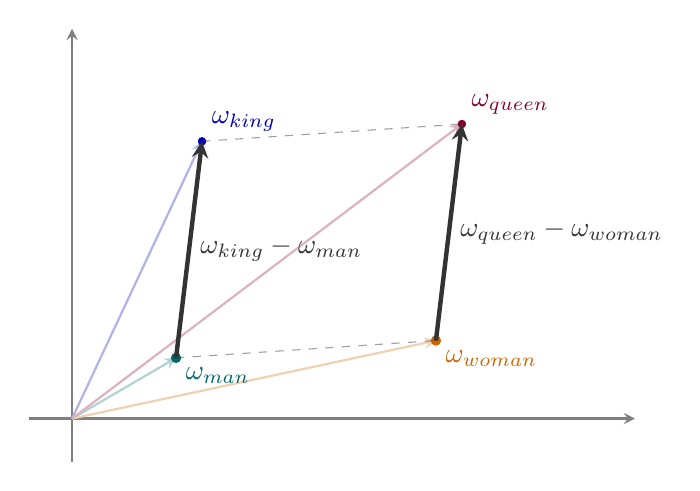
\begin{tikzpicture}[>=stealth, scale=1.1, font=\sffamily]

        % Farbendefinitionen (mit Schwarz abgedunkelt, damit sie professionell und nicht grell wirken)
        \colorlet{colorMan}{teal!80!black}      % Abgedunkeltes Blaugrün
        \colorlet{colorKing}{blue!70!black}     % Abgedunkeltes Blau
        \colorlet{colorWoman}{orange!80!black}  % Rostrot/Dunkelorange
        \colorlet{colorQueen}{purple!70!black}  % Abgedunkeltes Lila

        % Define axes
        \draw[->, thick, gray] (-0.5, 0) -- (6.5, 0); 
        \draw[->, thick, gray] (0, -0.5) -- (0, 4.5); 

        % Define coordinates
        \coordinate (O) at (0,0);
        \coordinate (man) at (1.2, 0.7);
        \coordinate (king) at (1.5, 3.2);
        \coordinate (woman) at (4.2, 0.9);
        \coordinate (queen) at (4.5, 3.4);

        % --- 1. Subtle Vectors from Origin (Background) ---
        % Die Vektoren vom Ursprung bekommen die jeweilige Farbe, aber sehr hell/transparent (!30)
        \draw[->, thick, colorMan!30] (O) -- (man);
        \draw[->, thick, colorKing!30] (O) -- (king);
        \draw[->, thick, colorWoman!30] (O) -- (woman);
        \draw[->, thick, colorQueen!30] (O) -- (queen);

        % --- 2. Points and Labels (Foreground) ---
        % Die Punkte und die Bezeichnungen in der kräftigen Farbe
        \filldraw[colorMan] (man) circle (1.5pt) node[below right] {$\boldsymbol{\omega}_{\text{man}}$};
        \filldraw[colorKing] (king) circle (1.2pt) node[above right] {$\boldsymbol{\omega}_{\text{king}}$};
        \filldraw[colorWoman] (woman) circle (1.5pt) node[below right] {$\boldsymbol{\omega}_{\text{woman}}$};
        \filldraw[colorQueen] (queen) circle (1.2pt) node[above right] {$\boldsymbol{\omega}_{\text{queen}}$};

        % --- 3. Relational Vectors (The Subtraction/Algebra) ---
        % Die algebraischen Pfeile in neutralem Dunkelgrau, um Kontrast zu den bunten Punkten zu schaffen
        \draw[->, ultra thick, black!80] (man) -- (king) 
            node[midway, right, xshift= 0.0cm] {$\boldsymbol{\omega}_{\text{king}} - \boldsymbol{\omega}_{\text{man}}$};
            
        \draw[->, ultra thick, black!80] (woman) -- (queen) 
            node[midway, right, xshift=0.0cm] {$\boldsymbol{\omega}_{\text{queen}} - \boldsymbol{\omega}_{\text{woman}}$};

        % Dashed horizontal connections to imply the parallelogram
        \draw[dashed, darkgray, opacity=0.5] (man) -- (woman);
        \draw[dashed, darkgray, opacity=0.5] (king) -- (queen);

    \end{tikzpicture}
    \caption[Geometric visualization of word vector algebra.]{Geometric visualization of the algebraic word analogy. The parallel translation vectors illustrate that the geometric difference $\boldsymbol{\omega}_{\text{king}} - \boldsymbol{\omega}_{\text{man}}$ is approximately equal to $\boldsymbol{\omega}_{\text{queen}} - \boldsymbol{\omega}_{\text{woman}}$, which enables arithmetic operations within the semantic vector space. (Own illustration)}
    \label{fig:embedding_analogy}
\end{figure}

% A notable extension of the static paradigm is FastText by \citet{Bojanowski2017}, which decomposes each token into a bag of overlapping character $n$-grams and represents the token as the sum of its constituent $n$-gram vectors. This sub-word decomposition provides two key advantages over purely word-level methods. First, it enables meaningful representations for tokens that were never observed during training (\ac{OOV} tokens), since their $n$-grams will typically overlap with those of known tokens. Second, it is particularly well suited for morphologically rich languages such as German, where productive compounding generates a combinatorial explosion of surface forms. A compound noun like \enquote{Einkommensteuererklärung} (income tax return) may never appear in the training corpus as a single vocabulary entry, yet FastText can construct a meaningful representation from its constituent $n$-grams that overlap with those of \enquote{Einkommen}, \enquote{Steuer} and \enquote{Erklärung} \citet{Bojanowski2017}.

%% -----  contextualized embeddings; e.g. ELMo, BERT, etc. 

\paragraph{Contextual Semantic Embeddings.}
\label{sec:contextual_embeddings}

A major deficit of these static embedding methods is their static nature and context independence. Once training is complete, the matrix $\mathbf{\Omega}$ is fixed and each token $w_i$ is consistently mapped to the exact same vector $\boldsymbol{\omega}_i$ regardless of its surroundings. The resulting semantic distortion is particularly obvious for homonyms and polysemes, since different word meanings will collapse into a single representation \cite{ethayarajh-2019-contextual}\cite[p. 174 f.]{Jurafsky2024_SLP} eg. the word \emph{book} will have the same embedding whether it refers to a physical object or the act of reserving something. Contextualized embedding models address this limitation by dynamically conditioning token representations on their surrounding context \cite[p.~174~f.]{Jurafsky2024_SLP}\cite{peters_2018_deep}.

Formally, any sequence of $n$ tokens $W = (w_1, \dots, w_n)$ is no longer processed through independent, fixed lookups. Instead, an embedding model maps the entire sequence jointly into a matrix of contextualised token representations $\phi_{\boldsymbol{\theta}}(W) = [\mathbf{e}_1, \dots, \mathbf{e}_n] = \mathbf{E} \in \mathbb{R}^{d \times n}$, where each vector $\mathbf{e}_i$ depends not only on the identity of token $w_i$ but on all other tokens in the sequence. Consequently, the same token receives different representations in different contexts, directly resolving the polysemy and homonymy problem that static methods cannot address \cite{peters_2018_deep,ethayarajh-2019-contextual}.

The foundational breakthrough enabling this dynamic representation was the introduction of the Transformer architecture by \citet{Vaswani2017}. As a deep neural network, the Transformer is composed of multiple stacked layers that progressively refine the input representations, but unlike its recurrent and convolutional predecessors, it entirely forgoes sequential processing in favour of a fully parallelisable mechanism known as self-attention \cite[p. 357 f.]{Bishop2024}. Intuitively, self-attention is the process of determining, for each token in the sequence, which other tokens are relevant to it and how strongly they should influence its representation \cite[p. 357 f.]{Bishop2024}\cite[p. 208 f.]{Goldberg2017}\cite{Vaswani2017}. 

Because self-attention processes all tokens simultaneously as an unordered set, it inherently lacks any notion of sequential order. To inject positional information, the input tokens are first mapped to initial static semantic token embeddings $\tilde{\mathbf{E}}$ and enriched with positional encodings $\mathbf{P} \in \mathbb{R}^{d \times n}$, producing $\mathbf{E}_{\text{in}} = \tilde{\mathbf{E}} + \mathbf{P}$ as the input to the Transformer layers \cite[p. 174 f.]{Jurafsky2024_SLP}\cite[p. 213 f.]{prince2023understanding}\cite{Vaswani2017}. A single self-attention layer transforms $\mathbf{E}_{\text{in}}$ by applying three learned linear projections to produce the Query ($\mathbf{Q}$), Key ($\mathbf{K}$) and Value ($\mathbf{V}$) matrices:

\vspace{-1em}
\[
\mathbf{Q} = \mathbf{W}_Q^\top \mathbf{E}_{\text{in}}, \quad  \mathbf{K} = \mathbf{W}_K^\top \mathbf{E}_{\text{in}}, \quad  \mathbf{V} = \mathbf{W}_V^\top \mathbf{E}_{\text{in}},
\]
\vspace{-1em}

where $\mathbf{W}_Q, \mathbf{W}_K, \mathbf{W}_V \in \mathbb{R}^{d \times d_k}$ are trainable weight matrices \cite[p. 212 f.]{prince2023understanding}\cite{Vaswani2017}. These projections serve different roles in the attention mechanism. The Query vector of a given token encodes what information this token is looking for, while the Key vectors characterise what each other token represents. The dot product between a Query and all Keys yields attention scores that quantify the relevance of each sequence position to the querying token. These scores are then used to compute a weighted sum over the Value vectors, which carry the actual content that each token contributes to the output \cite[p. 362 f.]{Bishop2024}\cite{Vaswani2017}. The full operation is formalised as scaled dot-product attention

\vspace{-1em}
\[
\mathrm{Attn}(\mathbf{Q},\mathbf{K},\mathbf{V}) = \mathrm{softmax}\!\left(\frac{\mathbf{Q}^\top \mathbf{K}}{\sqrt{d}}\right)\mathbf{V}.
\]
\vspace{-1em}

The scaling factor $\sqrt{d}$ prevents the dot products from growing large enough to push the softmax into regions of vanishing gradients, while the softmax normalisation ensures that the resulting weights form a probability distribution over the sequence. Each token's output representation is thus a weighted combination of all Value vectors in the sequence, where contextually relevant tokens receive higher weights \cite[p. 366 f.]{Bishop2024}\cite[p. 214]{prince2023understanding}\cite{Vaswani2017}.

To increase the representational capacity, multiple such attention operations are computed in parallel, a mechanism known as Multi-Head Attention. Allowing the model to attend to different types of relationships simultaneously e.g., syntactic dependencies in one head, semantic associations in another \cite{rogers_2020_bertology}. The outputs of all heads are concatenated and linearly projected back to the model dimension \cite[p. 366 f.]{Bishop2024}\cite[p. 176 f.]{Jurafsky2024_SLP}\cite{Vaswani2017}. Each Transformer layer further comprises residual connections that preserve information from earlier layers, layer normalisation that stabilises training and a position-wise feedforward network that enables the learning of more complex, non-linear patterns. By stacking multiple such layers, the Transformer builds increasingly abstract, contextualised representations that capture both local syntactic patterns and long-range semantic dependencies \cite[p. 191 f.]{Jurafsky2024_SLP}\cite{Vaswani2017}\cite{rogers_2020_bertology}.

The original Transformer was designed as an encoder-decoder architecture for sequence-to-sequence tasks such as machine translation \cite[p. 208 f.]{Goldberg2017}\cite{Vaswani2017}. The encoder transforms the input sequence into contextualised representations, while the decoder generates the output sequence token by token \cite[p. 198 f.]{Goldberg2017}\cite{Vaswani2017}. Further research has indicated that each component can be used independently, giving rise to two model families. Decoder-only models e.g., the GPT family by \citet{radford_improving_2018} employ causal (left-to-right) self-attention to generate text autoregressively \cite[p. 383 f.]{Bishop2024}. In contrast, encoder-only models employ bidirectional self-attention across the full input sequence. This makes them particularly well suited for tasks that require rich contextual representations of existing text rather than the generation of new text \cite[p. 388 f.]{Bishop2024}\cite{devlin_2019_bert}.

The most prominent encoder-only model is \ac{BERT} by \citet{devlin_2019_bert}. To learn its bidirectional representations, \ac{BERT} is trained through two self-supervised objectives \cite[p. 219 f.]{prince2023understanding}.  The primary task is \ac{MLM}, where a random subset of input tokens (15\%) is selected, of which 80\% are replaced by a special [MASK] token, 10\% by a random token and 10\% are left unchanged. The model is then trained to reconstruct the original tokens based on the entire surrounding context, which is formalised as the maximisation of the conditional probability of the masked tokens $\mathcal{M}  \subseteq \{1, \dots, n\}$ given an unmasked sequence $\max_\theta \prod_{i \in \mathcal{M}} \mathbb{P}_\theta(w_i | W_{\setminus \mathcal{M}})$ \cite[p. 388]{Bishop2024}\cite[p. 202 f.]{Jurafsky2024_SLP}\cite{devlin_2019_bert}. The second training task, Next Sentence Prediction, trains the model to determine whether two given sentences are consecutive in the original text, thereby encouraging the learning of cross-sentence coherence \cite[p. 204 f.]{Jurafsky2024_SLP}\cite{devlin_2019_bert}. Together, these objectives enable \ac{BERT} to learn contextualised representations $\mathbf{E_{\text{out}}} = [\mathbf{e}_1, \dots, \mathbf{e}_n]$ that encode intra-sentence semantics as well as inter-sentence relationships \cite{rogers_2020_bertology}.

Following \ac{BERT}, many architectural variations and refinements have been proposed, including RoBERTa by \citet{liu2019roberta}, which optimises the training procedure on larger corpora and DeBERTa by \citet{he2021debertadecodingenhancedbertdisentangled}, which detaches content and positional information in the attention mechanism. But all share the defining property that each token's representation is a dynamic function of its entire sequence context \cite[p. 207 f.]{Jurafsky2024_SLP}.

%% --- Pooling

\subsection{Sequence Embeddings}

For many applications, token-level representations are insufficient and a single, fixed-dimensional vector that captures the meaning of an entire sequence is required. To achieve this, an aggregation function $\psi$ can be applied to the matrix of token embeddings $\mathbf{E}$ to produce a single sequence embedding $\mathbf{z} = \psi(\mathbf{E}) \in \mathbb{R}^d$ \cite{xing2025comparative}. 

There are two aggregation strategies that are prevalent in practice. On the one hand, [CLS]-pooling extracts the representation of the special classification token prepended to the input:

\begin{equation}
    \mathbf{z}_{\texttt{[CLS]}} = \mathbf{e}_{\texttt{[CLS]}}
    \label{eq:cls_pooling}
\end{equation}

While architecturally convenient, this representation is trained for next-sentence prediction in \ac{BERT} or not explicitly trained at all in RoBERTa and has been shown to perform poorly on semantic similarity tasks without dedicated fine-tuning \cite{reimers2019sentence,devlin_2019_bert,Li_2020_Sentence}.

On the other hand, mean-pooling computes the average over all token representations

\begin{equation}
    \mathbf{z}_{\text{mean}} = \frac{1}{|\mathcal{T}|} 
    \sum_{i \in \mathcal{T}} \mathbf{e}_i
    \label{eq:mean_pooling}
\end{equation}

where $\mathcal{T} \subseteq \{1, \ldots, n\}$ denotes the set of token indices. \citet{reimers2019sentence} empirically demonstrate that mean-pooling consistently outperforms \texttt{[CLS]}-pooling for encoders that have not been fine-tuned for sentence-level tasks.

However, even with mean-pooling, representations from vanilla pre-trained encoders yield suboptimal sentence embeddings, since the aggregation is applied to representations that were never trained to encode sequence-level semantics \cite{reimers2019sentence, Li_2020_Sentence}. To address this, \citet{reimers2019sentence} proposed Sentence-\ac{BERT}, which fine-tunes the encoder using a Siamese architecture with a contrastive objective on natural language inference labels, producing sequence embeddings $\mathbf{z}$ where cosine similarity directly reflects semantic relatedness. \citet{gao-etal-2021-simcse} later demonstrated with SimCSE that comparable quality can be achieved through simpler contrastive objectives, using dropout augmentation as a minimal positive-pair generator. 


%One common approach is mean pooling, which computes the average of the token embeddings across the sequence $ \mathbf{z} = \frac{1}{n} \sum_{i=1}^n \mathbf{e}_i $ \cite{xing2025comparative}. 

%Another approach is to use the output of a special classification token (e.g., [CLS] in BERT) as the sequence embedding, although this has been shown to perform poorly on semantic similarity tasks without task-specific fine-tuning \cite{reimers2019sentence}. To address this, Sentence-BERT fine-tunes the model using a siamese architecture and a contrastive loss based on natural language inference labels, resulting in sequence embeddings where cosine similarity directly reflects semantic relatedness \cite{reimers2019sentence}[src].
%(\cite{gao-etal-2021-simcse})

\subsection{Similarity Measures}

The ultimate goal of learning structured representation spaces is to enable the use of geometric operations to capture semantic relationships \cite{Mikolov2013}. The most fundamental operation is the measurement of similarity or distance between two vectors $\mathbf{z}_1, \mathbf{z}_2 \in \mathbb{R}^d$. Common similarity measures include, the Euclidean distance $d(\mathbf{z}_1, \mathbf{z}_2) = \sqrt{\sum_{i=1}^d (z_{1i} - z_{2i})^2}$, which captures absolute distance in the vector space and the cosine similarity $\mathrm{sim}(\mathbf{z}_1, \mathbf{z}_2) = \frac{\mathbf{z}_1^\top \mathbf{z}_2}{\|\mathbf{z}_1\| \|\mathbf{z}_2\|}$, which measures the angle between two vectors and is invariant to their magnitude \cite[p. 103 f., p. 112 f.]{Jurafsky2024_SLP}\cite[p. 48 f.]{Goldberg2017}. As illustrated in Figure \ref{fig:similarity_measures}, the choice of similarity measure can significantly impact downstream tasks such as retrieval, clustering, or classification, as it defines the geometric notion of semantic relatedness in the embedding space \cite{manning2008introduction,reimers2019sentence}.


\begin{figure}[htpb]
    \centering
    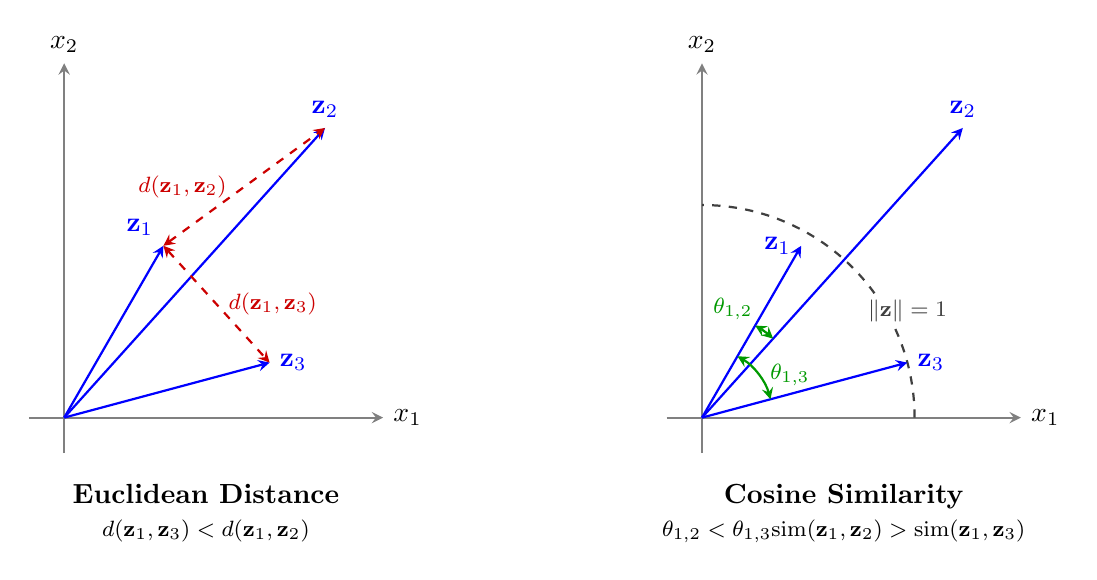
\begin{tikzpicture}[>=stealth, scale=0.9, font=\sffamily]

        % ==========================================
        % LEFT PANEL: Euclidean Distance
        % ==========================================
        \begin{scope}[xshift=-4.5cm]
            % Axes
            \draw[->, thick, gray] (-0.5, 0) -- (4.5, 0) node[right, text=black] {$x_1$};
            \draw[->, thick, gray] (0, -0.5) -- (0, 5) node[above, text=black] {$x_2$};

            % Coordinates using Polar (Angle:Radius) for perfect spacing
            \coordinate (z1) at (60:2.8);
            \coordinate (z2) at (48:5.5);
            \coordinate (z3) at (15:3.0);

            % Vectors
            \draw[->, thick, blue] (0,0) -- (z1) node[above left] {$\mathbf{z}_1$};
            \draw[->, thick, blue] (0,0) -- (z2) node[above] {$\mathbf{z}_2$};
            \draw[->, thick, blue] (0,0) -- (z3) node[right] {$\mathbf{z}_3$};

            % Euclidean Distances with white background for text readability
            \draw[<->, thick, red!80!black, dashed] (z1) -- (z2) 
                node[midway,left, inner sep=6pt, font=\footnotesize] {$d(\mathbf{z}_1, \mathbf{z}_2)$};
            \draw[<->, thick, red!80!black, dashed] (z1) -- (z3) 
                node[midway, right, inner sep=4pt, font=\footnotesize] {$d(\mathbf{z}_1, \mathbf{z}_3)$};

            % Objective statement
            \node[below, font=\bfseries] at (2.0, -0.8) {Euclidean Distance};
            \node[below, text=black, font=\footnotesize] at (2.0, -1.3) {$d(\mathbf{z}_1, \mathbf{z}_3) < d(\mathbf{z}_1, \mathbf{z}_2)$};
        \end{scope}

        % ==========================================
        % RIGHT PANEL: Cosine Similarity
        % ==========================================
        \begin{scope}[xshift=4.5cm]
            % Axes
            \draw[->, thick, gray] (-0.5, 0) -- (4.5, 0) node[right, text=black] {$x_1$};
            \draw[->, thick, gray] (0, -0.5) -- (0, 5) node[above, text=black] {$x_2$};

            % Coordinates (Identical to left panel)
            \coordinate (z1) at (60:2.8);
            \coordinate (z2) at (48:5.5);
            \coordinate (z3) at (15:3.0);

            % Unit Circle projection
            \draw[dashed, darkgray, thick] (3.0,0) arc (0:90:3.0);
            \node[darkgray, font=\footnotesize, fill=white, inner sep=1pt] at (2.9, 1.5) {$\|\mathbf{z}\| = 1$};

            % Vectors
            \draw[->, thick, blue] (0,0) -- (z1) node[left] {$\mathbf{z}_1$};
            \draw[->, thick, blue] (0,0) -- (z2) node[above] {$\mathbf{z}_2$};
            \draw[->, thick, blue] (0,0) -- (z3) node[right] {$\mathbf{z}_3$};

            % Angles with white backgrounds for readability
            \draw[<->, thick, green!60!black] (48:1.5) arc (48:60:1.5) 
                node[midway, above left, font=\footnotesize, inner sep=4pt] {$\theta_{1,2}$};
            \draw[<->, thick, green!60!black] (15:1.0) arc (15:60:1.0) 
                node[midway, right, xshift=2pt, font=\footnotesize, inner sep=2pt] {$\theta_{1,3}$};

            % Objective statement
            \node[below, font=\bfseries] at (2.0, -0.8) {Cosine Similarity};
            \node[below, text=black, font=\footnotesize] at (2.0, -1.3) {$\theta_{1,2} < \theta_{1,3} \implies \mathrm{sim}(\mathbf{z}_1, \mathbf{z}_2) > \mathrm{sim}(\mathbf{z}_1, \mathbf{z}_3)$};
        \end{scope}

    \end{tikzpicture}
    \caption[Comparison of Euclidean distance and cosine similarity.]{Geometric comparison of similarity measures. Depending on the chosen metric, the resulting similarity rankings diverge: In the Euclidean space (\textbf{left}), $\mathbf{z}_1$ is considered more similar to $\mathbf{z}_3$ due to their spatial proximity, as the metric is sensitive to vector magnitudes. Conversely, the cosine similarity (\textbf{right}) evaluates only the angular alignment ($\theta$), identifying $\mathbf{z}_1$ and $\mathbf{z}_2$ as the most similar pair. (Own illustration)}
    \label{fig:similarity_measures}
\end{figure}

%\subsection{further Embedding Technologies}
%... (bspw. graph embeddings, multimodale Embeddings, etc.)
